\chapter{Reputation Availability}
\label{chap:rep_avail}
The incentive system's goal is to provide a good level of service to those peers
who abide by the rules of the system. Since the system measures this via a
reputation point system, reputation must be available to cooperative peers.
That is, they must be able to gain the required amount of reputation within a
reasonable time frame and maintain it afterwards. At the same time, they should
not be so quickly contented with their level of reputation that they frequently
lose the incentive to participate. This chapter examines under which
circumstances this is the case using the simulation described in
Chapter~\ref{chap:implementation}.

\section{Setup}
This chapter contains evaluations of many simulation runs. The simulation uses
\texttt{.settings} files for configuration that make the results reproducible.
For each simulation run in this chapter a name of the corresponding
\texttt{.settings} file is given. These are distributed along with the
implementation in the \texttt{thesis/simulation\_runs/} subdirectory.

The simulation runs are based on the default configuration
(\texttt{default.settings}). The most relevant parameters are listed in the
appendix (Section~\ref{sec:app_default_settings}) along with a short
explanation. For detailed information on the meaning of the parameters, see
Chapter~\ref{chap:implementation}.

Simulations last 200 seconds.

\section{Peer Selection Strategy}
\label{sec:selection}
Many requests or incoming queries make it necessary for a peer to send a query
to a query peer. The peer must then choose the recipient of the query. How peers
choose influences the reputation availability in the system. A number of
different strategies have been implemented, three of which are presented in the
following.

In the simulations, the strategy under examination is used by all peers.

\subsection{Strategy: \emph{Overlap}}
\label{sec:rep_avail_selection_overlap}
This is the default selection strategy that was described in the
Section~\ref{sec:desc_querying}. Out of all possible recipients, the peer
chooses one whose routing prefix overlaps maximally with the target ID (overlap
of two bit strings is also defined in Section~\ref{sec:desc_querying}). Under
the assumption that peers have complete subprefix coverage, this ensures that
queries always terminate and no routing loops occur, since at each hop the
distance to the target ID shrinks.

The strategy does not specify a tie breaker. In the simulation, query groups are
maintained as Python \texttt{OrderedDict} objects, which are always iterated
over in a predictable order. Upon entering a query group, this object is copied
to the new member, so that he also has the same iteration order. This leads to a
problem where some "lucky" peers always get picked first, simply because of
their position in the dictionary. Others in contrast have a difficult time
getting any reputation because they don't receive queries (they may still
receive some though, e.g. after the first choice failed).

Figure~\ref{fig:selection_overlap_peer_reps} shows examples of a peer (on the
left) who is "lucky" in one query group (not so much in others, but he can still
get by), and another (on the right) who is unable to gain sufficient reputation.
Other peers not shown are able to quickly gain reputation in all their groups.

An example of the effect on the reputation percentiles in a query group is shown
in figure~\ref{fig:selection_overlap_rep_percs}: the 50th percentile and above
can easily gain reputation, while peers below struggle.

The underlying problem is that peers have no consideration for which peers could
use queries in order to gain reputation. There end up being "rich" peers and
"poor" peers because of this.

While this is caused by an artifact of the implementation, it is by no means
certain that this problem couldn't occur in a real system. Peers may use an
implementation that also tends to favor some peers over others for lack of a tie
breaker.

\begin{figure}[t]
\centering
\includegraphics[width=0.5\columnwidth]{figures/selection_overlap_peer_reps_3_of_64}%
\includegraphics[width=0.5\columnwidth]{figures/selection_overlap_peer_reps_5_of_64}
\captionsettings{Reputation over time for strategy \emph{overlap} for 2
peers}{selection\_strategy/selection\_overlap.settings}
\label{fig:selection_overlap_peer_reps}
\end{figure}

\begin{figure}[t]
\centering
\includegraphics[width=1\columnwidth]{figures/selection_overlap_rep_percs_2_of_14}
\captionsettings{Reputation percentiles over time for strategy \emph{overlap} in
one query group}{selection\_strategy/selection\_overlap.settings}
\label{fig:selection_overlap_rep_percs}
\end{figure}

Figure~\ref{fig:selection_overlap_resp_statuses} shows the response statuses
over time. They are fairly well-behaved, with timeouts and unmatched responses
that settle at a low level.

\begin{figure}[t]
\centering
\includegraphics[width=1\columnwidth]{figures/selection_overlap_resp_statuses}
\captionsettings{Response statuses over time for strategy
\emph{overlap}}{selection\_strategy/selection\_overlap.settings}
\label{fig:selection_overlap_resp_statuses}
\end{figure}

\subsection{Strategy: \emph{Overlap $\rightarrow$ Reputation Saturated Last}}
This strategy is a modification of the \emph{overlap} strategy, but with a
secondary criterion as a tie breaker. Peers still start out choosing a recipient
based on the overlap, but they give potential recipients who they assume to be
reputation saturated a lower priority than those who they assume are not.

Effectively, the peer makes a list of all eligible query peers and sorts it by
the overlap length, longest first. Then he goes through the list and takes out
any potential recipient who is reputation saturated and appends him to the back.
The peer at the beginning of the list is then chosen. Any peer that is not
reputation saturated will be chosen over peers that are.

The rationale is that a reputation saturated recipient would not
bother responding, so the peer himself has an incentive to not choose that
recipient. As a side effect, it's supposed to shift queries away from those
peers that were chosen first with the \emph{overlap} strategy towards those who
were "unlucky".

The peer of course doesn't know exactly whether a potential recipient is
reputation saturated, since this is a policy decision up to the recipient. But
he can guess the potential recipient's saturation reputation. In the simulation,
peers assume a potential recipient is saturated if they would be in his
position.

This strategy is based on the \emph{overlap} strategy and offers almost the same
protection against routing loops. One situation in which they can occur anyway
is if all peers with
a higher overlap are saturated. In that case, a peer with equal or lower overlap
is chosen.

Figure~\ref{fig:selection_overlap_high_rep_last_rep_percs} shows the reputation
percentiles of 2 query groups. The ability for peers of the lowest percentiles
to gain reputation compares favorably to the \emph{overlap} strategy, they are
able to eventually pass the penalty threshold. However, they take much longer to
do it than peers of the higher percentiles. Both of these observations were to
be expected, since "unlucky" peers, who previously were not selected, are now
given priority once the "lucky" ones are reputation saturated. But this takes
some time, explaining the delay for the lower percentiles.

\begin{figure}[t]
\centering
\includegraphics[width=0.5\columnwidth]{figures/selection_overlap_high_rep_last_rep_percs_1_of_14}%
\includegraphics[width=0.5\columnwidth]{figures/selection_overlap_high_rep_last_rep_percs_4_of_14}
\captionsettings{Reputation percentiles over time for strategy \emph{overlap
$\rightarrow$ reputation saturated last} in 2 query
groups}{selection\_strategy/selection\_overlap\_high\_rep\_last.settings}
\label{fig:selection_overlap_high_rep_last_rep_percs}
\end{figure}

Figure~\ref{fig:selection_overlap_high_rep_last_peer_reps} shows the reputation
development of 2 peers. On the left, an example of a peer gaining quickly in one
group, but with a delay in another. On the right, an extreme example for whom
reputation gains in all groups is delayed for a long time, but happens
eventually. There are also examples of peers able to gain reputation quickly in
all groups not shown here.

\begin{figure}[t]
\centering
\includegraphics[width=0.5\columnwidth]{figures/selection_overlap_high_rep_last_peer_reps_1_of_64}%
\includegraphics[width=0.5\columnwidth]{figures/selection_overlap_high_rep_last_peer_reps_24_of_64}
\captionsettings{Reputation over time for strategy \emph{overlap $\rightarrow$
reputation saturated last} for 2
peers}{selection\_strategy/selection\_overlap\_high\_rep\_last.settings}
\label{fig:selection_overlap_high_rep_last_peer_reps}
\end{figure}

Figure~\ref{fig:selection_overlap_high_rep_last_resp_statuses} shows the
response statuses over time. Compared with the \emph{overlap} strategy, there
are a few more timeouts and unmatched queries. The difference isn't big, and can
be explained by the possibility of selecting unsuitable peers.

\begin{figure}[t]
\centering
\includegraphics[width=1\columnwidth]{figures/selection_overlap_high_rep_last_resp_statuses}
\captionsettings{Response statuses over time for strategy \emph{overlap
$\rightarrow$ reputation saturated
last}}{selection\_strategy/selection\_overlap\_high\_rep\_last.settings}
\label{fig:selection_overlap_high_rep_last_resp_statuses}
\end{figure}

\subsection{Strategy: \emph{Overlap $\rightarrow$ Reputation Sorted}}
\label{sec:rep_avail_selection_overlap_rep_sorted}
This strategy is another modification of the \emph{overlap} strategy. The
querying peer again starts with all eligible query peers sorted by the overlap
length. As a tie breaker he uses the reputation the potential recipient has in
any shared query group, lowest first. So effectively, out of all potential
recipients he will only consider the subset consisting of those whose overlap is
greatest and chose the one with the lowest reputation.

The strategy was designed to address the issue with \emph{overlap $\rightarrow$
reputation saturated last}, namely that "unlucky" peers still have to wait for
the "lucky" ones to become reputation saturated before they can gain reputation
at a practical rate. By selecting the lowest-reputation peer within the group
with maximal overlap, the ability to gain reputation should be better
distributed among all peers.

It is of course still required for a peer to be useful to others in the query
group, i.e. be in the group with maximal overlap in the first place.

Figure~\ref{fig:selection_overlap_rep_sorted_rep_percs} shows reputation
percentiles in 2 query groups. One in which reputation is gained easily by all
peers, one in which the 5th percentile can't quite maintain the penalty
threshold reputation for a while. This is due to one peer suffering from the
recursive query problem. At around time 150, this peer gains above the penalty
threshold reputation in his last query group and the problems go away.

\begin{figure}[t]
\centering
\includegraphics[width=0.5\columnwidth]{figures/selection_overlap_rep_sorted_rep_percs_2_of_15}%
\includegraphics[width=0.5\columnwidth]{figures/selection_overlap_rep_sorted_rep_percs_3_of_15}
\captionsettings{Reputation percentiles over time for strategy \emph{overlap
$\rightarrow$ reputation sorted} in 2 query
groups}{selection\_strategy/selection\_overlap\_rep\_sorted.settings}
\label{fig:selection_overlap_rep_sorted_rep_percs}
\end{figure}

Figure~\ref{fig:selection_overlap_rep_sorted_peer_reps} shows the reputation
development of 2 peers. The one on the left has it very easy to gain reputation,
the one on the right struggles for a while in 2 of his 3 query groups, but can
eventually gain and maintain beyond the penalty threshold reputation. This is
one the worst cases as well, if you exclude peers that are members of very small
query groups in which reputation gains are slow simply because of the low amount
of traffic.

The left graph very clearly shows a sort of sawtooth pattern that stems from the
peer letting a query time out once he is reputation saturated at 14 reputation,
thus falling down to 12 and subsequently starting to gain reputation again.

\begin{figure}[t]
\centering
\includegraphics[width=0.5\columnwidth]{figures/selection_overlap_rep_sorted_peer_reps_11_of_64}%
\includegraphics[width=0.5\columnwidth]{figures/selection_overlap_rep_sorted_peer_reps_56_of_64}
\captionsettings{Reputation over time for strategy \emph{overlap $\rightarrow$
reputation sorted} for 2
peers}{selection\_strategy/selection\_overlap\_rep\_sorted.settings}
\label{fig:selection_overlap_rep_sorted_peer_reps}
\end{figure}

The frequencies of response statuses presented in
figure~\ref{fig:selection_overlap_rep_sorted_resp_statuses} shows this
strategy to be better than the other \emph{overlap} strategies in terms of query
success rate.

\begin{figure}[t]
\centering
\includegraphics[width=1\columnwidth]{figures/selection_overlap_rep_sorted_resp_statuses}
\captionsettings{Response statuses over time for strategy \emph{overlap
$\rightarrow$ reputation
sorted}}{selection\_strategy/selection\_overlap\_rep\_sorted.settings}
\label{fig:selection_overlap_rep_sorted_resp_statuses}
\end{figure}

\emph{Overlap $\rightarrow$ reputation sorted} is the best performing of the
strategies presented here for the purpose of reputation availability.
Essentially all peers can quickly and reliably gain reputation (again
disregarding peers in very small query groups, since that is just a problem with
the simplified implementation).

It also prevents routing loops as well as any, since the querying peer always
picks a recipient from the group of peers with maximal overlap. In this regard,
it is clearly better than \emph{overlap $\rightarrow$ reputation saturated
last}, where this was not necessarily the case.

\section{Reputation Attenuation}
\label{sec:attenuation}
An important performance characteristic of the DHT which the reputation system
supports is the likelihood that a peer responds to a query. Since we're assuming
all peers are selfish and inherently lazy, this is by no means guaranteed.

In the settings for the simulation used here, the penalty threshold is 10 and
the reputation buffer is 4. That means peers play nice and gather reputation
until they are reputation saturated at 14 reputation, then decide that they have
enough. The next time they're required to do something, e.g. respond to a query,
they ignore this, incurring a penalty. Thus they are not saturated anymore, so
they cooperate until they are again.

The amount of cooperative actions a peer has to perform to get back up to his
saturation reputation ultimately determines his response probability. It is
determined by the magnitude of the penalty he receives when he drops below his
saturation reputation and that of the rewards he receives as he works his way
back up. So the response probability of the system can be adjusted via the
penalties and rewards. If we assume the only reward of magnitude $r$ is given
for successfully responding and the only penalty of magnitude $p$ is given for
not responding at all, peers need to earn $\frac{p}{r}$ rewards for every
penalty they receive. The response probability that can be expected is thus
$\frac{p}{p + r}$.

So the probability could be controlled via the penalties and rewards, and it
should work reasonably well if all peers are already well-established in the
system above the penalty threshold. But with larger differences between
reward and penalty, it becomes very difficult for a newcomer to become
established.

Doing this also only works assuming that peers don't make unintentional
mistakes. Such mistakes, called \emph{trembles} can e.g. be due to unusual
delays or failures in the network. If peers are unlucky and tremble repeatedly,
without being able to make up for it in between, this may crash their
reputation.

The recursive query problem may then make it impossible for them (or for
newcomers) to become established. For example, assuming a target response
probability of 95\%, the ratio of reward to penalty would have to be 1:19, so
newcomers would have to earn more than 19 rewards for every penalty they incur
in order to make progress towards the penalty threshold.

Removing the penalty threshold (i.e. setting it to 0) is also not an option,
since the purpose of it is to prevent whitewashing by requiring newcomers to put
in some work before enjoying unpenalized service. The solution presented here is
to make a distinction between two phases. In the first, a peer works to
establish himself in the system while having less than the penalty threshold
reputation. The second phase is the steady state after where he maintains his
reputation. In the first phase, reputation is gained as usual, but in the
second, reputation earnings are attenuated by one of two strategies presented
here. Their purpose is to allow the regulation of the response probability
without impacting newcomers' ability to establish themselves.

A distinction is made between \emph{raw reputation} $r_r$ and \emph{effective
reputation} $r_e$, where \emph{raw reputation} is the reputation as previously,
and \emph{effective reputation} is the result of applying an attenuation
function $att$ to the raw reputation. The effective reputation is what is used
when a decision has to be made based on a peer's reputation, e.g. how much of a
penalty delay to impose.

When updating a peer's reputation, rewards are applied to the raw reputation,
while penalties are applied to the effective reputation:

When a reward, i.e. a reputation update changing the reputation by an amount
$r_{diff} > 0$, is applied to a peer with effective reputation $r_e$, the
effective reputation is set to $att(att^{-1}(r_e) + r_{diff})$. So essentially
the raw reputation is calculated from the effective reputation, then the update
applied, and the result turned back into effective reputation.

When a penalty, i.e. a reputation update changing the reputation by an amount
$r_{diff} < 0$, is applied to a peer with effective reputation $r_e$, the
effective reputation is set to $r_e - r_{diff}$.

With these differing rules for rewards and penalties it is possible to make it
increasingly harder for peers to gain effective reputation the more they already
have, while maintaining the same threat for misbehavior.

In both of the strategies, there is an \emph{attenuation threshold}, which is
the amount of reputation below which reputation is unmodified, i.e. $att$ is the
identity function for input values below the threshold. That threshold is the
same as the penalty threshold in all examples given here. An upper limit on the
reputation which peers can't surpass is also implemented, but has no influence
since peers don't reach it in the simulations.

\subsection{Strategy: \emph{Constant}}
The first strategy simply multiplies all raw reputation above the threshold by a
fixed coefficient $c$. $t$ is the reputation threshold, $l$ the upper reputation
limit.

\[att_{const}(r_r) = min(min(r_r, t) + c \cdot max(r_r - t, 0), l)\]

\begin{figure}[t]
\centering
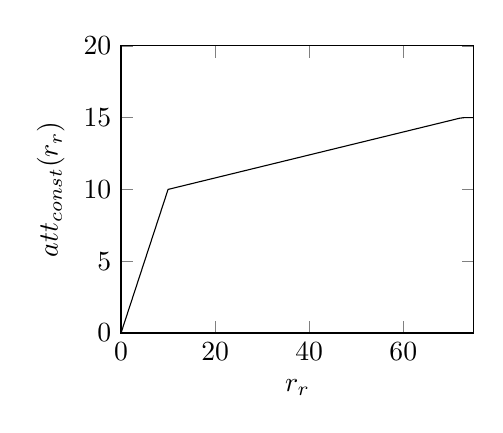
\begin{tikzpicture}
\begin{axis}[
    xlabel=$r_r$,
    ylabel={$att_{const}(r_r)$},
    xmin=0,
    xmax=75,
    ymin=0,
    ymax=20,
    width=0.5\columnwidth
]
\addplot[domain=0:75, samples=76]{min(min(x, 10) + 0.08 * max(x - 10, 0), 15)};
\end{axis}
\end{tikzpicture}%
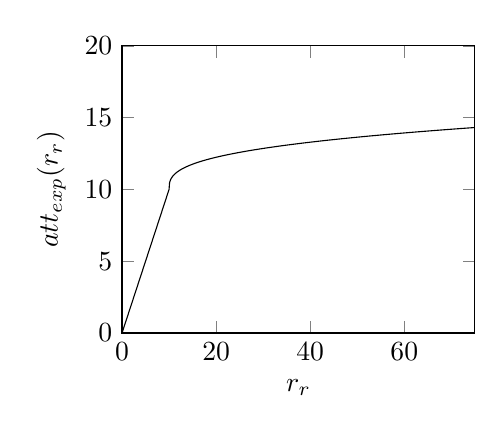
\begin{tikzpicture}
\begin{axis}[
    xlabel=$r_r$,
    ylabel={$att_{exp}(r_r)$},
    xmin=0,
    xmax=75,
    ymin=0,
    ymax=20,
    width=0.5\columnwidth
]
\addplot[domain=0:75, samples=751]{min(min(x, 10) + max(x - 10, 0) ^ 0.35, 15)};
\end{axis}
\end{tikzpicture}
\caption{Raw vs. effective reputation for \emph{constant} attenuation ($t$ = 10,
$c = 0.08$, $l = 15$) on the left and \emph{exponential} ($t$ = 10, $p = 0.35$,
$c = 1$, $l = 15$) on the right.}
\label{fig:att_raw_vs_eff}
\end{figure}

\subsection{Strategy: \emph{Exponential}}
The other strategy raises all raw reputation above the threshold to a fixed
power $p$ and multiplies the result by a coefficient $c$. $t$ is the reputation
threshold, $l$ the upper reputation limit.

\[att_{exp}(r_r) = min(min(r_r, t) + c \cdot max(r_r - t, 0)^p, l)\]

\subsection{Comparison}
Figures~\ref{fig:attenuation_percs} and \ref{fig:attenuation_resp} show
reputation percentiles and response statuses of simulation runs demonstrating
the different attenuation strategies. The percentiles are all of the same query
group, with the same members. The example was chosen to illustrate a few points.
It is not representative of the overall performance, many other groups perform
better.

The parameters in the attenuated simulations have been chosen so that it takes
roughly the same amount of raw reputation to get from 10 (the attenuation
threshold) to 14 (the saturation reputation for all peers): $\frac{4}{0.08} =
50$ for \emph{constant}, and $4^{\frac{1}{0.35}} \approx 52.5$ for
\emph{exponential}. In effect, the first peers to become saturated in the
attenuated cases do so at around the same time.

\begin{figure}[t]
  \centering
  \begin{subfigure}[t]{0.45\columnwidth}
    \centering
    \includegraphics[width=\columnwidth]{figures/attenuation_no_attenuation_rep_percs_1_of_15}
    \subcaptionsettings{No
    attenuation}{attenuation/attenuation\_no\_attenuation.settings}
    \label{fig:attenuation_no_att_percs}
  \end{subfigure}\hfill%
  \begin{subfigure}[t]{0.45\columnwidth}
    \centering
    \includegraphics[width=\columnwidth]{figures/{{attenuation_0.08_constant_rep_percs_1_of_15}}}
    \subcaptionsettings{\emph{Constant} attenuation, $c =
    0.08$}{attenuation/attenuation\_0.08\_constant.settings}
    \label{fig:attenuation_constant_percs}
  \end{subfigure}\hfill\\%
  \begin{subfigure}[t]{0.45\columnwidth}
    \centering
    \includegraphics[width=\columnwidth]{figures/{{attenuation_0.35_1_exponential_rep_percs_1_of_15}}}
    \subcaptionsettings{\emph{Exponential} attenuation, $p = 0.35$, $c =
    1$}{attenuation/attenuation\_0.35\_1\_exponential.settings}
    \label{fig:attenuation_exp_percs}
  \end{subfigure}\hfill%
  \caption{Reputation percentiles in the same query group for different
  attenuation strategies. For the attenuated, $t = 10$ and $l = 15$.}
  \label{fig:attenuation_percs}
\end{figure}

\begin{figure}[t]
  \centering
  \begin{subfigure}[t]{0.45\columnwidth}
    \centering
    \includegraphics[width=\columnwidth]{figures/attenuation_no_attenuation_resp_statuses}
    \subcaptionsettings{No
    attenuation}{attenuation/attenuation\_no\_attenuation.settings}
    \label{fig:attenuation_no_att_resp}
  \end{subfigure}\hfill%
  \begin{subfigure}[t]{0.45\columnwidth}
    \centering
    \includegraphics[width=\columnwidth]{figures/{{attenuation_0.08_constant_resp_statuses}}}
    \subcaptionsettings{\emph{Constant} attenuation, $c =
    0.08$}{attenuation/attenuation\_0.08\_constant.settings}
    \label{fig:attenuation_constant_resp}
  \end{subfigure}\hfill\\%
  \begin{subfigure}[t]{0.45\columnwidth}
    \centering
    \includegraphics[width=\columnwidth]{figures/{{attenuation_0.35_1_exponential_resp_statuses}}}
    \subcaptionsettings{\emph{Exponential} attenuation, $p = 0.35$, $c =
    1$}{attenuation/attenuation\_0.35\_1\_exponential.settings}
    \label{fig:attenuation_exp_resp}
  \end{subfigure}\hfill%
  \caption{Response statuses for different attenuation strategies. For the
  attenuated, $t = 10$ and $l = 15$.}
  \label{fig:attenuation_resp}
\end{figure}

Without attenuation, oscillation can be seen in the reputation percentiles,
which reflects oscillation in individual peer reputations. Peers are also
getting significantly above the reputation at which they are saturated (14). The
reason is that, while peers expect penalties (see
Section~\ref{sec:penalty_expectations}), they do not expect rewards. This leads
to them answering multiple queries in a row, even though answering only the
first would have made them saturated; the reputation update simply hasn't
arrived yet. This is of course still true for the attenuated cases, but here it
takes a lot more raw reputation to get to the saturated effective reputation.

\emph{Constant} and \emph{exponential} attenuation differ slightly. In the
former, every point of raw reputation is attenuated in the same way, while in
the latter the attenuation increases as the peer's accumulated effective
reputation rises. Attenuation just above the threshold (between 10 and 11) is
actually negative, i.e. the effective reputation yielded is greater than the raw
reputation. The attenuation gets stronger after that. This makes it easier for
peers to gain reputation just above the penalty threshold in order to be able to
tolerate a tremble. This is demonstrated by the simulations: the 5th percentile
(the struggling peer) manages to reliably stay above the penalty threshold with
\emph{exponential} attenuation (figure~\ref{fig:attenuation_exp_percs}), while
he dips below it once more for the \emph{constant} case
(figure~\ref{fig:attenuation_constant_percs}). And the 25th percentile is also
"stuck" at around the penalty threshold for a lot longer in the \emph{constant}
case.

\begin{figure}[t]
\centering
\includegraphics[width=1\columnwidth]{{{figures/attenuation_0.0417_constant_12_threshold_rep_percs_6_of_15}}}
\captionsettings{Reputation percentiles over time for \emph{constant}
attenuation with higher threshold ($c = 0.0417$, $t =
12$)}{attenuation/attenuation\_0.0417\_constant\_12\_threshold.settings}
\label{fig:attenuation_0.0417_constant_12_threshold_percs}
\end{figure}

A possibility to address this is to set the attenuation threshold above the
penalty threshold, allowing peers to e.g. gain enough reputation to tolerate a
tremble without attenuation kicking in. This is shown in
figure~\ref{fig:attenuation_0.0417_constant_12_threshold_percs}: \emph{constant}
attenuation is used but the threshold is set to 12, and the coefficient is
adjusted to 0.0417, so that it still takes 50 raw reputation to get from 10 to
14 effective reputation. The struggling peer's reputation develops in a way
comparable to \emph{exponential} or \emph{harmonic} from
figure~\ref{fig:attenuation_percs}.

A potential problem with this approach is that the rules of the system must make
an assumption about how many trembles a peer should be able to tolerate and set
the attenuation threshold appropriately. In order to achieve the same expected
response probability, effective reputation above the higher threshold has to be
more "expensive". However, if some peer is satisfied with being able to tolerate
fewer trembles than the system assumes, he may get away with no attenuation at
all. In the example shown in
figure~\ref{fig:attenuation_0.0417_constant_12_threshold_percs}, the threshold
is set so peers can easily get to 12 reputation, where they are able to tolerate
one penalty of 2 points. A peer may be confident he won't drop below 10
reputation once he reaches it, and ignore queries once he reaches 12 reputation.
That peer would never have his reputation attenuated and have a very low
response probability.

On the other hand, \emph{exponential} attenuation is disadvantageous for peers
who want to be able to tolerate more trembles for extra reliability, since
effective reputation gets more and more expensive. For example, using
\emph{exponential} attenuation with $c = 1$, $p = 0.35$ (as in the examples), it
takes about 52.5 raw reputation to get from 10 to 14 effective reputation. In
order to get from 10 to 16 (being able to tolerate 3 trembles), it takes 167.2.
This puts a much higher stress on such peers wishing for more reliability.

A solution to this could be to cap the "cost" of effective reputation,
essentially combining \emph{exponential} attenuation with \emph{constant}
attenuation, switching over to the latter once a certain amount of effective
reputation has been earned.

The reputation cap (the upper limit of effective reputation that can't be
surpassed) is meant to ensure activity in the query groups by preventing peers
from collecting a lot of reputation up front and then not responding to queries
for prolonged periods. In the simulations, this didn't become relevant because
all peers let queries time out once 14 effective reputation are reached. With
\emph{exponential} attenuation, it's not a viable strategy anyway, since
effective reputation gets more and more expensive. But with \emph{constant}
attenuation an upper limit may well become necessary.

Figure~\ref{fig:attenuation_resp} shows the response statuses for the
simulations corresponding to the reputation percentiles in
figure~\ref{fig:attenuation_percs}. \emph{Constant} attenuation is quite similar
to \emph{exponential}, but has a few more timeouts. This is due to the fact that
it takes less raw reputation to get from 12 to 14 than for the other attenuation
strategies (25 compared to 45.26 and 42, respectively). That means after letting
an incoming query time out, peers can work their way back up to 14 faster.

Without attenuation, there are many more timeouts, and as a consequence also
many more messages in total. Here, peers are very easily able to earn 14
reputation and become saturated, at which point they let the next query time
out. This is the reason attenuation is necessary.

\section{Penalty Expectations}
\label{sec:penalty_expectations}
Reputation attenuation, introduced in Section~\ref{sec:attenuation}, as well as
penalty expectations, described in the following, are enabled in the default
settings. When both are disabled, quite severe oscillations in individual peer
reputations can be observed that are also reflected in reputation percentiles of
query groups.

\begin{figure}[t]
\centering
\includegraphics[width=0.5\columnwidth]{figures/expectations_off_no_att_peer_reps_3_of_64}%
\includegraphics[width=0.5\columnwidth]{figures/expectations_off_no_att_rep_percs_1_of_15}
\captionsettings{Reputation oscillation of a peer and in the percentiles of a
query group with penalty expectations and reputation attenuation
off}{penalty\_expectations/expectations\_off\_no\_att.settings}
\label{fig:penalty_expectations_off_no_att_peer_reps_percs}
\end{figure}

Figure~\ref{fig:penalty_expectations_off_no_att_peer_reps_percs} demonstrates
this. The peer's reputation shown on the left fluctuates heavily, going down to
or even below the penalty threshold of 10. This is in spite of the fact that the
peers in the simulation try to stay above it. These oscillations are also
visible in the per-query-group reputation percentiles shown on the right.

This is because peers aren't taking into account that reputation updates take
some time to be disseminated. They only respond to an incoming query if they are
not reputation saturated. Once they let a query time out, the penalty they will
receive is not applied immediately, due to the timeout on the side of the sender
and the network delay. So peers think they are still reputation saturated and
let following queries time out as well, until the first penalty hits. By that
time, several penalties may have accrued which will be applied thereafter,
crashing their reputation. In the peer reputation in
figure~\ref{fig:penalty_expectations_off_no_att_peer_reps_percs} it can be seen
that reputation decreases usually happen all at once after the peer has
surpassed the saturation reputation of 14.

\begin{figure}[t]
\centering
\includegraphics[width=0.5\columnwidth]{figures/expectations_off_no_att_high_buf_peer_reps_3_of_64}%
\includegraphics[width=0.5\columnwidth]{figures/expectations_off_no_att_high_buf_rep_percs_1_of_15}
\captionsettings{Reputation oscillation at a higher base level with increased
reputation buffer of
20}{penalty\_expectations/expectations\_off\_no\_att\_high\_buf.settings}
\label{fig:penalty_expectations_off_no_att_high_buf_peer_reps_percs}
\end{figure}

A workaround for this is to increase peer's reputation buffers. This results in
an outcome shown in
figure~\ref{fig:penalty_expectations_off_no_att_high_buf_peer_reps_percs}, where
the buffer has been increased from 4 to 20, meaning peers only let queries time
out once they have accumulated 30 reputation, rather than 14. Both peer
reputations and percentiles look similar, but have been shifted to a higher
level. Peers' reputations still fluctuate, but because of the higher buffer
doesn't dip below the penalty threshold of 10 anymore.

However, this is not a good solution because then the amount of buffer a peer
needs depends on the amount of queries he is likely to receive within a short
time (the time between the first defecting action and the corresponding penalty
arriving). Peers would need to adjust the buffer based on the activity in the
query group. Some strategies for reputation attenuation presented in
Section~\ref{sec:attenuation} also make it more difficult to gain reputation for
a peer the more he already has, so he may have to do much more work than
necessary.

The better solution to the problem is to make peers expect to receive a penalty
when they do something they know is going to be penalized, and make their
decisions based on their reputation with expected penalties already applied. In
the implementation, peers make these expectations when they purposefully let a
query time out, and when they send a fail response.

The implementation actually isn't ideal, as peers cannot expect timeout
penalties due to the recursive query problem: When peer A queries peer B, B may
need to query peer C in order to serve the query. If that second query to C
takes so long that A's query times out, ideally B would expect a timeout
penalty. However, this is not implemented, and expecting a penalty once the
response from C arrives doesn't make sense, since at that point the penalty has
likely already been applied.

\begin{figure}[t]
\centering
\includegraphics[width=0.5\columnwidth]{figures/expectations_on_no_att_peer_reps_3_of_64}%
\includegraphics[width=0.5\columnwidth]{figures/expectations_on_no_att_rep_percs_1_of_15}
\captionsettings{Reduced reputation oscillation with expectations enabled, but
attenuation still
disabled}{penalty\_expectations/expectations\_on\_no\_att.settings}
\label{fig:penalty_expectations_on_no_att_peer_reps_percs}
\end{figure}

Figure~\ref{fig:penalty_expectations_on_no_att_peer_reps_percs} shows the result
of enabling penalty expectations, while reputation attenuation is still
disabled. Peers are now able to stay above the penalty threshold without a large
buffer.

To clarify, enabled penalty expectations are part of the default settings and
were used in the other simulations in this chapter.

\subsection{Impact of Attenuation}
Keeping penalty expectations disabled but enabling reputation attenuation also
significantly improves the behavior of the system.

\begin{figure}[t]
\centering
\includegraphics[width=0.5\columnwidth]{figures/expectations_off_peer_reps_16_of_64}%
\includegraphics[width=0.5\columnwidth]{figures/expectations_off_rep_percs_1_of_15}
\captionsettings{Reputation of one peer and percentiles of a query group with
just attenuation enabled, expectations
off}{penalty\_expectations/expectations\_off.settings}
\label{fig:penalty_expectations_off_peer_reps_percs}
\end{figure}

Figure~\ref{fig:penalty_expectations_off_peer_reps_percs} gives an example of
this. The reputation percentiles of the query group selected for it show almost
all peers of the query group managing to stay above the penalty threshold almost
all of the time. At first glance this suggests that penalty expectations are
unnecessary if reputation attenuation is enabled.  However, the problem solved
by penalty expectations still exists when just attenuation is used: the
individual reputations of the peer on the left show him dipping below the
penalty threshold just after he became reputation saturated.

Rather, the reason just adding attenuation already looks a lot more tidy is that
it takes peers a lot longer to become reputation saturated. These are the
trigger points when peers without expectations let more queries time out than
they should. With fewer of them, peers don't lose reputation as often, making
their reputation much more stable.

\section{Recursive Query Problem}
\label{sec:rep_avail_rec_query_prob}
The recursive query problem is described in
Section~\ref{sec:desc_rec_query_prob}.  In it, a peers low reputation in one
query group causes trouble in another.  Figure~\ref{fig:rec_query_prob}
illustrates this: It shows the reputation of a peer who is a member in three
query groups. In two of them, he gains reputation quite quickly and gets above
the penalty threshold. But in the other, his reputation gains are a little
delayed. The two gray bars show that around time 25 where his reputation in the
third group is still below the penalty threshold, he suffers from the recursive
query problem for a fraction of his responses.  During that time, he can't gain
reputation in his first two groups because he needs the third group to respond
quickly enough. But once his reputation in that group passes the penalty
threshold, the problems stop.

\begin{figure}[t]
\centering
\includegraphics[width=1\columnwidth]{figures/selection_overlap_rep_sorted_peer_reps_with_rqp_29_of_64}
\captionsettings{Peer reputations showing the recursive query
problem}{selection\_strategy/selection\_overlap\_rep\_sorted.settings}
\label{fig:rec_query_prob}
\end{figure}

\section{Joining a Running Network}
In the simulations presented so far, all peers are added at the beginning with
no reputation. But one important characteristic the system needs is that it must
be possible for a newcomer to join a running system in which the peers have
already established themselves.

This hasn't been examined in great detail, but one simulation has been run for
200 simulated seconds with mostly the default settings, except that in addition
to the 64 peers added at the beginning, 16 peers each are added at time 50, 100,
and 150.

\begin{figure}[t]
\centering
\includegraphics[width=0.5\columnwidth]{figures/3_times_16_rep_percs_12_of_31}%
\includegraphics[width=0.5\columnwidth]{figures/3_times_16_resp_statuses}
\captionsettings{Reputation percentiles of one query group and response statuses
for a simulation with late joiners}{established/3\_times\_16.settings}
\label{fig:3_times_16}
\end{figure}

Figure~\ref{fig:3_times_16} shows the reputation percentiles of a query group
in which some peers join later than others, as well as response statuses.
They both show that, under these conditions, joining late is fine. The
percentiles drop each time new peers without reputation join, but they are all
able to gain reputation, all ending up well above the penalty threshold. The
number of timeouts and unmatched queries settles at low level.

The fact this works so well may be in part due to two peculiarities of the
implementation. Firstly, the mechanism for finding query groups makes it more
likely that newcomers share a group, where the recursive query problem is not
much of an issue, because no one expects good service yet.

Secondly, the routing prefix is quite short at 4 bits. This means a high chance
peers are able to answer a query from local knowledge because they happen to be
in the correct sync group. If this becomes less likely, the recursive query
problem may become more pronounced.

\section{Effect of Small Sync Groups}
\label{sec:rep_avail_small_sync_groups}
One major cause of concern that was revealed by the simulation is related to
sync groups with very few or even no members. If there are any of them, the
system becomes very brittle.

The problem with empty sync groups is that there are no authoritative peers for
the corresponding routing prefix. There will be queries for that prefix sent by
peers looking to complete their subprefix coverage, but no one to tell them that
no peer exists with that prefix. The recipients always have to send a fail
response and incur the penalty for it. Since these queries are sent repeatedly,
this continues and crashes their reputation.

But even if care is taken that each sync group contains at least one peer, the
system is brittle.

\begin{figure}[t]
\centering
\includegraphics[width=0.5\columnwidth]{{{figures/256_steady_8_prefix_0.05_delay_rep_percs_25_of_89}}}%
\includegraphics[width=0.5\columnwidth]{{{figures/256_steady_8_prefix_0.05_delay_peer_reps_with_rqp_236_of_256}}}
\captionsettings{Reputation percentiles and peer reputations showing brittleness
with small sync
groups}{large\_sims/256\_steady\_8\_prefix\_0.05\_delay.settings}
\label{fig:brittleness}
\end{figure}

Figure~\ref{fig:brittleness} shows examples of reputation percentiles and peer
reputations in a simulation with 256 peers and a routing prefix length of 8 bits
(i.e. every peer is his own sync group).

Everything starts out looking quite good, but at one point the reputation of
some peers in the depicted query group and all the reputations of the depicted
peer crash. That point is when the first peers reach their saturation
reputation.

What probably happens is that these peers ignore the next incoming query, and
then the peers who were supposed to receive the response are unable to answer
their own query for which they needed that response. This only needs to happen
twice and their reputation dips below the penalty threshold. Then the recursive
query problem takes over: There are still peers with high reputation who expect
fast responses, but the peers with low reputation are unable to provide them.

It isn't clear why this only happens with small sync groups. It could have to do
with the fact that with more sync peers, there is a choice of who to query.

Then again, it may not have to do with the small sync groups directly, but with
the longer routing prefix. This requires more hops to resolve a query, which
means more chances for a timeout to occur.

The reason is unknown, but the issue could in all instances be prevented by
reducing the routing prefix length, thereby increasing the average number of
peers per sync group.

\section{Tit-for-Tat}
A very simple and effective strategy in game theory is tit-for-tat: when
employing it, the player essentially treats another player he interacts with the
same way he is being treated. He starts out cooperating with the other player,
but if he is betrayed, he defects.

Something resembling this strategy can be used within query groups. The rewards
and penalties can be set so that any peer has either zero reputation or the
penalty threshold reputation. A peer is then given either maximal or no penalty
delay, depending on his last action.

It is very easy for peers to gain and maintain reputation, since they only need
to perform one cooperative action. But they also can't ever defect, or they'll
be penalized during their next query. Very quickly, all peers are only
cooperating.

In fact, this still works if there is 5\% chance of peers trembling and not
responding to a query by accident. Figure~\ref{fig:tft_trembles_peer_reps} shows
one peer's reputations during such a simulation. He regularly trembles and all
of his reputation is removed.

\begin{figure}[t]
\centering
\includegraphics[width=1\columnwidth]{{{figures/tft_trembles_peer_reps_with_rqp_5_of_64}}}
\captionsettings{One peer's reputations when using tit-for-tat with
trembles}{tit-for-tat/tft\_trembles.settings} \label{fig:tft_trembles_peer_reps}
\end{figure}

The recursive query problem then makes it difficult to answer queries which the
peer needs to forward. However, it takes only one query for a record the peer is
responsible for (which he can answer without having to ask anyone else) to get
him back to the penalty threshold. This happens regularly, so that the peer
spends most of his time with high reputation. Although with a longer routing
prefix the chance of that happening drops.

These rules seem good in this respect, but the all-or-nothing nature likely make
them unsuitable when the system is fully implemented. It is not possible to give
a higher penalty for timeouts than for fail responses, so there is no incentive
to send them. It is also impossible to give only a small reward for the upkeep
operations like broadcasting reputation updates.
